\section{Optimisation for Processor Architectures
\label{sec:pa}}

\subsection{NVIDIA GPU}
The LFRic-microbenchmark suite~\cite{lfric-microbenchmarks} allows
optimisations for individual kernels to be explored without having to
compile and run the whole code. This is particularly useful when
targeting a programming model such as OpenACC for GPU architectures
where the Portland group compiler cannot compile the Fortran 2003 used 
in the main code.

The local matrix assembly (LMA) matrix-vector kernel had been
previously ported to run on GPUs by inserting OpenACC directives in
the PSy layer code to control the data transfer from host memory to
device memory and to offload the kernel call to the GPU device. This
OpenACC version was the starting point for Alan Gray from NVIDIA to
to look at optimisations. Moreover, after discussions regarding 
the PSyKAl API and the LFRic plans for how OpenACC will be
implemented for a GPU version, NVIDIA believe that the plan and
implementation will enable a successful GPU implementation.
This is a summary of potential optimisations from NVIDIA.

\begin{lstlisting}[language=Fortran,caption={Code fragment of original 
    kernel},label={lst:LMA-orig}]
  !$acc loop vector 
  do k = 0, nlayers-1
    lhs_e(:,:) = 0.0_r_def
    ik = (cell-1)*nlayers + k + 1

    do df = 1, ndf1
      do df2 = 1, ndf2
        lhs_e(df,k) = lhs_e(df,k) + & 
          matrix(df,df2,ik)*x(map2(df2)+k)
      end do
    end do

    do df = 1, ndf1
      lhs(map1(df)+k) = lhs(map1(df)+k) + lhs_e(df,k)
    end do

  end do  
\end{lstlisting}

Shown in listing~\ref{lst:LMA-orig} is a code fragment of the LMA
kernel. It has an OpenACC directive \verb+!$acc loop vector+ before the
outermost $k$ loop, so that each thread in a thread block will do different loop
iterations. This code runs on a GPU, but not very efficiently. 

The first optimisation was to fuse the two loops over \verb+ndf1+
(lines 6-11 and 13-15) and replace the array \verb+lhs_e+ with a
scalar. The scalar can stay resident in a register for each thread and
avoids unnecessary memory accesses. This optimisation is called loop
fuse. 

The second optimisation was to exploit more parallelism on the GPU.
This performed with the OpenACC loop clause {\em collapse} to combine
the two outermost loops. This has the added benefit of aiding {\em
  memory coalescence}, {\em i.e.} neighbouring parallel threads
accessing neighbouring memory locations. However, an OpenACC {\em
  atomic update} directive is required as the loop over {\em ndf1} is
now also parallel. This optimisation is called Loop collapse. The new
kernel code is shown in listing~\ref{lst:LMA-opt}. 

\begin{lstlisting}[language=Fortran,caption={Optimised
    kernel},label={lst:LMA-opt}]
  !$acc loop vector collapse(2)
  do k = 0, nlayers-1
    do df = 1, ndf1

      ik = (cell-1)*nlayers + k + 1
      lhs_e_scal = 0.0_r_def

      do df2 = 1, ndf2
         lhs_e_scal = lhs_e_scal + & 
            matrix(df,df2,ik)*x(map2(df2)+k)
      end do
      
      !$acc atomic update
      lhs(map1(df)+k) = lhs(map1(df)+k) + lhs_e_scal

    end do
  end do
\end{lstlisting}

These first two optimisations increase the speed of execution but the
code still has a large register usage which results in low occupancy
of the GPU parallel units. This can be reduced by inlining the kernel
subroutine into the PSy layer. This can be done by the PGI compiler,
using Inter-procedural Analysis (IPA). This triggered by the following
compiler flag \verb+-Mipa=inline:reshape -Minfo flags+. The info flag
is for reporting purposes. This optimisation is called Inlining. 

The final optimisation is to note that the kernel is launched multiple
times, as the PSy layer includes the colouring ordering code for serialisation
to prevent race conditions. The kernel executes faster with a
single launch and NVIDIA optimised this by loop collapsing the loop
over colours and cells per colour. In the full code, this could be
simply done by not colouring at all. This optimisation is called
Single Kernel.

The colouring serialisation loop order is done for correctness,
however, the presence of the atomic update in the kernel prevents the
data race that colouring is designed to prevent, so the code is thread
safe. However, the atomic update doesn't guarantee the order of
execution, whereas colouring does. This means that whilst the data
race is avoided with the atomic update, the answer is not reproducible against
multiple runs. This is an optimisation which could be chosen for speed
when reproducibility is not an issue.

Shown in Table~\ref{tab:lma_nvidia} are the execution times for each
optimisation and in figure~\ref{fig:lma_nvidia} is shown the resulting
speed up versus the original code version.

\begin{table}
\centering
\caption{\label{tab:lma_nvidia} Execution times for different
  optimisations of a single run of  the LMA kernel on an V100 
  {\em Volta} NVIDIA GPU.}
\begin{tabular}{rc}
Optimisation & time (ms) \\\hline
Original     & $9.45$ \\
Loop fusion  & $5.33$ \\
Loop collapse & $2.68$ \\ 
Inlining      & $0.58$ \\
Single Kernel & $0.32$ \\\hline
\end{tabular}
\end{table}

\begin{figure}
\centering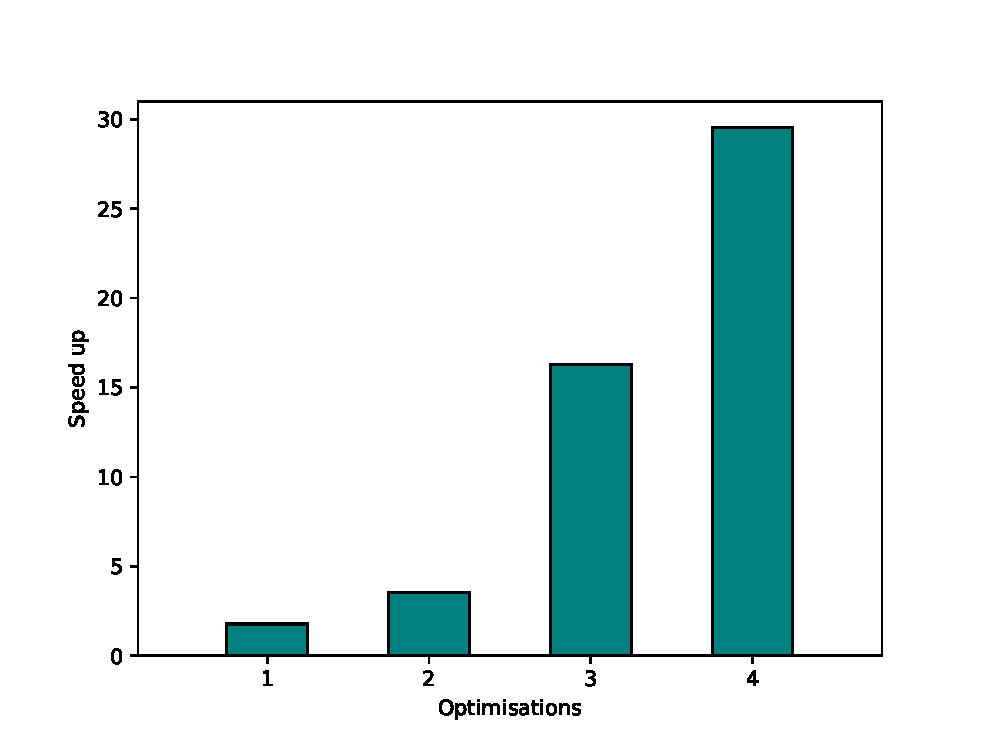
\includegraphics[width=1.0\linewidth]{figs/LMA-nvidia.eps}
\caption{\label{fig:lma_nvidia}Speed up of the LMA kernel against the
  original code for various optimisations. 1 loop fusion. 2 loop
  collapse. 3 Inlining. 4 Single Kernel.}
\end{figure} 

The speed up times are impressive, but a further analysis of the
absolute performance is useful. The NVIDIA profiler was
used to measure some performance metrics. This was compared to a simple ``roofline''
analysis~\cite{roofline} of the code on Volta. This suggests that as the arithmetic
intensity (flops per byte) of $0.3$ flops/byte of the kernel is low
compared to the ridge-line of the hardware, $9.9$ flops/byte, then the
code is memory bound. Comparing the memory bandwidth achieved of 549
GB/s to the Stream benchmark for the hardware suggests the code is
achieved around $70\%$ of the available bandwidth. This suggest the
code is fairly well optimised.

It should be noted that the problem size is too small, the data file
supplied to NVIDIA had $864$ cells with $40$ layers. Whilst, a target
local volume size of $12\times 12=144$ or $24\times 24=576$ is a
reasonable size for a single core of a CPU, a similar size is too
small to fully exploit the parallelism of GPU. In particular, to
effectively exploit the SIMT parallelism with the vertical degrees of
freedom, the vector size should be $128$ or more. $40$ levels is
clearly too few. Worse, in this particular case the colouring data here
had the non-optimal $6$ colours, whereas $4$ is sufficient. As seen in
the previous year's performance report the GPU should handle much more
work for a disproportional decrease in cost. This is especially true
for the number of levels.

These optimisations show that the code can run with some degree of
efficiency on a GPU. PSyclone is being developed so that is can
produce the necessary OpenACC directives in the PSy layer. Moreover,
its is being developed so that it can parse individual statements in
the kernel. This is necessary so that the kernel source can be
annotated with directives. Then the whole code can have a GPU
implementation generated automatically. To modify the actual source
code takes this a step further. However, it would in principle be
possible and moreover, this is similar to some of the ideas in CLAW~\cite{claw}.
CLAW is being considered for the parallelisation of the physical
parameterisations and some of the ideas would then be re-implemented in
PSyclone. Generating optimised code for GPUs is then possible.

